\begin{frame}
\frametitle{What is a graph}
\begin{itemize}
\pause
\item A bunch of vertices and a bunch of edges: \pause $G = (V, E)$

\inote{In math notation, this is two sets, one called $V$ and one called $E$}

\pause
\item Vertex: literally anything \inote{AKA `nodes'}

\pause
\item Edge: a set containing one or two vertices \inote {AKA `links'}

\inote{Why do we allow edges to have only one vertex? Could it have zero?}

\pause
\item We can draw graphs, but a drawing is just \alert{one interpretation} of a graph

\pause
\item Position doesn't matter, vertex-names do
\end{itemize}
\end{frame}

\begin{frame}
\frametitle{Undirected graph example}
\begin{example}
$$G = (\quad\{A, B, C, D\}, \quad \{\{A, B\}, \{A, B\}, \{C, D\}\} \quad)$$

\inote{Remember the picture is just one way of thinking about the graph.}

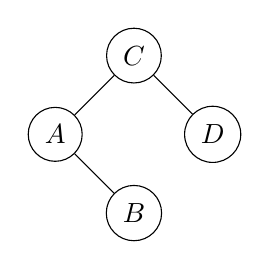
\begin{tikzpicture}
\node (A) at (0, 2) [circle,draw] {$A$};
\node (B) at (1, 1) [circle,draw] {$B$};
\node (C) at (1, 3) [circle,draw] {$C$};
\node (D) at (2, 2) [circle,draw] {$D$};
% \node (E) at (4, 2) [circle,draw] {$E$};

\draw (A) to (B);
\draw (A) to (C);
\draw (C) to (D);
% \draw (D) to [loop below] (D);
\end{tikzpicture}
\end{example}

\begin{itemize}
\pause
\item Vertices: \pause $A, B, C, D$ \inote{part of the definition}

\pause
\item Adjacent to $A$: \pause $B, C$

\pause
\item $\deg A$: \pause 2 \inote{because there are two edges incident to $A$}

\pause
\item Path from $B$ to $D$: \pause $[B, A, C, D]$


\pause
\item Any circuits? \pause no
\end{itemize}
\end{frame}

\begin{frame}
\frametitle{What can you do with an undirected graph?}
\begin{itemize}
\pause
\item Weighted graph (airline routes)

\pause
\item Bipartition: separate nodes into two categories such that every vertex in the first category only links to things in the second category, and vice-versa

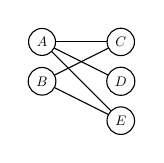
\begin{tikzpicture}[scale=0.5, every node/.style={scale=0.5}]
\node (A) at (0, -1) [circle,draw] {$A$};
\node (B) at (0, -2) [circle,draw] {$B$};
\node (C) at (2, -1) [circle,draw] {$C$};
\node (D) at (2, -2) [circle,draw] {$D$};
\node (E) at (2, -3) [circle,draw] {$E$};

\draw (A) to (C);
\draw (A) to (D);
\draw (A) to (E);
\draw (B) to (C);
\draw (B) to (E);
\end{tikzpicture}

\pause
\item Subgraph: If $G_1 = (V_1, E_1)$, then $G_2 = (V_2, E_2)$ where $V_1 \subseteq V_2$ and $E_1 \subseteq E_2$

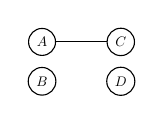
\begin{tikzpicture}[scale=0.5, every node/.style={scale=0.5}]
\node (A) at (0, -1) [circle,draw] {$A$};
\node (B) at (0, -2) [circle,draw] {$B$};
\node (C) at (2, -1) [circle,draw] {$C$};
\node (D) at (2, -2) [circle,draw] {$D$};

\draw (A) to (C);
\end{tikzpicture}

\inote{Is $G$ a subgraph of itself? Would $(\emptyset, \emptyset)$ be a subgraph of every graph?}

\pause
\item Union: if $G_1 = (V_1, E_1), G_2 = (V_2, E_2)$ then $G_1 \cup G_2 = (V_1 \cup V_2, E_1 \cup E_2)$

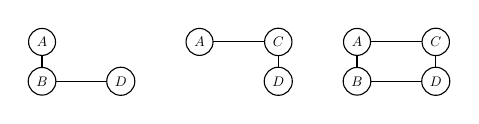
\begin{tikzpicture}[scale=0.5, every node/.style={scale=0.5}]
\node (A1) at (0, -1) [circle,draw] {$A$};
\node (B1) at (0, -2) [circle,draw] {$B$};
\node (D1) at (2, -2) [circle,draw] {$D$};

\draw (A1) to (B1);
\draw (B1) to (D1);

\node (A2) at (4, -1) [circle,draw] {$A$};
\node (C2) at (6, -1) [circle,draw] {$C$};
\node (D2) at (6, -2) [circle,draw] {$D$};

\draw (A2) to (C2);
\draw (C2) to (D2);

\node (A) at (8, -1) [circle,draw] {$A$};
\node (B) at (8, -2) [circle,draw] {$B$};
\node (C) at (10, -1) [circle,draw] {$C$};
\node (D) at (10, -2) [circle,draw] {$D$};

\draw (A) to (B);
\draw (A) to (C);
\draw (C) to (D);
\draw (B) to (D);
\end{tikzpicture}
\end{itemize}
\end{frame}


\begin{frame}
\frametitle{Special undirected graphs}
\begin{itemize}

\pause
\item Complete graph $K_n$: every vertex is connected to every other vertex

\begin{tikzpicture}[scale=0.5, every node/.style={scale=0.5,fill=blue}]
\input{complete_graph}
\end{tikzpicture}

\pause
\item Complete bipartite graph $K_{m,n}$: $m$ vertices connected to all $n$ vertices.

\begin{tikzpicture}[scale=0.5, every node/.style={scale=0.5,fill=blue}]
\begin{python}
m = 4
n = 6
max = 6

node_str = '\\node (A{i}) at ({x}, {y}) [circle,draw] {{}};\n'
for i in range(m):
    x, y = 10 / (m -  1) * i, 0
    print(node_str.format(**locals()))

node_str = '\\node (B{i}) at ({x}, {y}) [circle,draw] {{}};\n'
for i in range(n):
    x, y = 10 / (n - 1) * i, 2
    print(node_str.format(**locals()))

edge_str = '\\draw (A{i}) to (B{j});\n'
for i in range(m):
    for j in range(n):
        print(edge_str.format(**locals()))

\end{python}

%%% Local Variables:
%%% mode: latex
%%% TeX-master: "graphs"
%%% End:

\end{tikzpicture}
\end{itemize}
\end{frame}

\begin{frame}
\frametitle{Neat things you can do with graphs}
\begin{itemize}
\pause
\item Graph isomorphism: when two graphs would be the same if you could change the vertex labels
  \inote{The graphs don't have to be drawn in the same position; They could look totally different and still be isomorphic like these two:}

  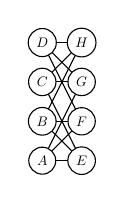
\begin{tikzpicture}[scale=0.5, every node/.style={scale=0.5}]
    \node (A) at (0, 0) [circle,draw] {$A$};
    \node (B) at (0, 1) [circle,draw] {$B$};
    \node (C) at (0, 2) [circle,draw] {$C$};
    \node (D) at (0, 3) [circle,draw] {$D$};
    \node (E) at (1, 0) [circle,draw] {$E$};
    \node (F) at (1, 1) [circle,draw] {$F$};
    \node (G) at (1, 2) [circle,draw] {$G$};
    \node (H) at (1, 3) [circle,draw] {$H$};
    \draw (A) to (E);
    \draw (A) to (F);
    \draw (A) to (G);
    \draw (B) to (E);
    \draw (B) to (F);
    \draw (B) to (H);
    \draw (C) to (E);
    \draw (C) to (G);
    \draw (C) to (H);
    \draw (D) to (F);
    \draw (D) to (G);
    \draw (D) to (H);
  \end{tikzpicture}
  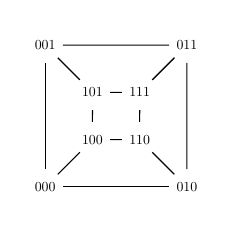
\begin{tikzpicture}[scale=0.6, every node/.style={scale=0.5}]
    \node (000) at (0, 0) [circle] {000};
    \node (001) at (0, 3) [circle] {001};
    \node (011) at (3, 3) [circle] {011};
    \node (010) at (3, 0) [circle] {010};
    \node (110) at (2, 1) [circle] {110};
    \node (100) at (1, 1) [circle] {100};
    \node (101) at (1, 2) [circle] {101};
    \node (111) at (2, 2) [circle] {111};

    \draw (000) to (001);
    \draw (000) to (010);
    \draw (000) to (100);
    \draw (011) to (010);
    \draw (011) to (001);
    \draw (011) to (111);
    \draw (111) to (110);
    \draw (111) to (101);
    \draw (111) to (011);
    \draw (101) to (100);
    \draw (101) to (001);
    \draw (110) to (100);
    \draw (110) to (010);
  \end{tikzpicture}

\pause
\item $k$-coloring: Color a graph such that no two vertices with the same color are touching each other. Try to use as few colors as possible.
  \inote{Can you think of a graph that takes $n$ colors to color?}

  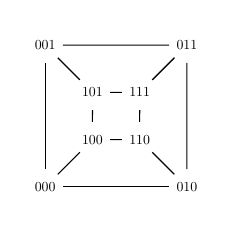
\begin{tikzpicture}[scale=0.6, every node/.style={scale=0.5}]
    \node (000) at (0, 0) [circle] {000};
    \node (001) at (0, 3) [circle] {001};
    \node (011) at (3, 3) [circle] {011};
    \node (010) at (3, 0) [circle] {010};
    \node (110) at (2, 1) [circle] {110};
    \node (100) at (1, 1) [circle] {100};
    \node (101) at (1, 2) [circle] {101};
    \node (111) at (2, 2) [circle] {111};

    \draw (000) to (001);
    \draw (000) to (010);
    \draw (000) to (100);
    \draw (011) to (010);
    \draw (011) to (001);
    \draw (011) to (111);
    \draw (111) to (110);
    \draw (111) to (101);
    \draw (111) to (011);
    \draw (101) to (100);
    \draw (101) to (001);
    \draw (110) to (100);
    \draw (110) to (010);
  \end{tikzpicture}
  \pause
  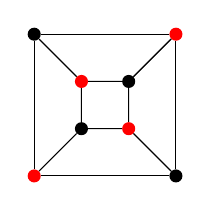
\begin{tikzpicture}[scale=0.6, every node/.style={scale=0.5}]
    \node (000) at (0, 0) [circle,fill=red] {};
    \node (001) at (0, 3) [circle,fill=black] {};
    \node (011) at (3, 3) [circle,fill=red] {};
    \node (010) at (3, 0) [circle,fill=black] {};
    \node (110) at (2, 1) [circle,fill=red] {};
    \node (100) at (1, 1) [circle,fill=black] {};
    \node (101) at (1, 2) [circle,fill=red] {};
    \node (111) at (2, 2) [circle,fill=black] {};

    \draw (000) to (001);
    \draw (000) to (010);
    \draw (000) to (100);
    \draw (011) to (010);
    \draw (011) to (001);
    \draw (011) to (111);
    \draw (111) to (110);
    \draw (111) to (101);
    \draw (111) to (011);
    \draw (101) to (100);
    \draw (101) to (001);
    \draw (110) to (100);
    \draw (110) to (010);
  \end{tikzpicture}
\end{itemize}
\end{frame}


\begin{frame}
\frametitle{Handshaking lemma}
\begin{theorem}
  Given $G = (V, E)$
  $$\sum_{v \in V} \deg v = 2\abs{E}$$
  % TODO: finish this
\end{theorem}
\end{frame}

%%% Local Variables:
%%% mode: latex
%%% TeX-master: "graphs"
%%% End:
